\chapter{Introduction} 
Organic semiconductors have a niche to fill across the landscape of electronic
device manufacturing due to the flexibility, processability, and cost of manufacturing. They have all ready
achieved commercial viability in organic light emitting
diodes (OLEDs) \cite{Song2020} and breakthroughs in organic field-effect transistors (OFETs)
indicate that that they are soon to folow \cite{Chen2020}. Exciting research is being done to provide stretchability, self-healing, and biodegradability for 
next generation medical devices \cite{Brutting2006}.
More generally, the solution processability of these materials allows for
cheaper manufacturing, the consumption of less rare elements, 
and the ability to assemble on curved substrates make the for a dizzying array of design possibilities. 
A survey of these materials, and a litany of
other emerging organic electronic technologies, can be found the survey text 
Organic Electronic: Emerging Concepts and Technologies
\cite{FabioCicoiraEditor2013}. 

The methods used in this thesis are centrally motivated by, and justified for, 
the application of our workflow to materials
used in the design of organic photovoltaics (OPVs) for use in organic solar cells (OSCs). However, the methods are
not exclusively applicable to these materials and could be applied similarly to  supplement the engineering of any organic
electronic devices, like those mentioned above. 
OSCs can assist us in harnessing the power of the sun in ways not available to traditional cells. 
For example, researchers have exploited a unique feature of the physics the excitonic photoabsorbtion in 
organic materials.  Namely, that absorbtion spectrum
in these materials is relatively narrow ($\approx$300nm)
With this, they are able to tune the active layer material to absorb radiation right above or right below the
visible spectrum (into the NIR or UV spectrum respectively). This 
could allow for the production of windows that passively draw current. Semi-transparent OSCs have already
reached 11 \% efficeincy \cite{Brabec2020}. 

In our present work, we present results from an investigation of two materials
used in the design of the active layer of organic solar cells (OSCs). P3HT, a
donor molecule, and ITIC, an acceptor molecule. With respect to organic electronic devices, `acceptors' are the
organic analogue of p-type inorganic semiconductors and `donors' the analogue
of the n-type.\ej{Good place for P3HT and ITIC figures. Also maybe a good place to talk about where they've been used before and how they're different.} We make this note because in the methods we describe a model of
a charge `hopping' from one molecule to another. And as we describe, our
investigation involves hops within a pure donor domain or within a pure
acceptor domain. A common point of confusion is distinguishing between which
molecules are donors or acceptors.
Any molecule can accept or donate a charge carrier.
They merely receive their donor/acceptor designation as a result of how they
are primarily utilized in electronic devices. 

\begin{figure}[]
\centering
\begin{subfigure}{.5\textwidth}
    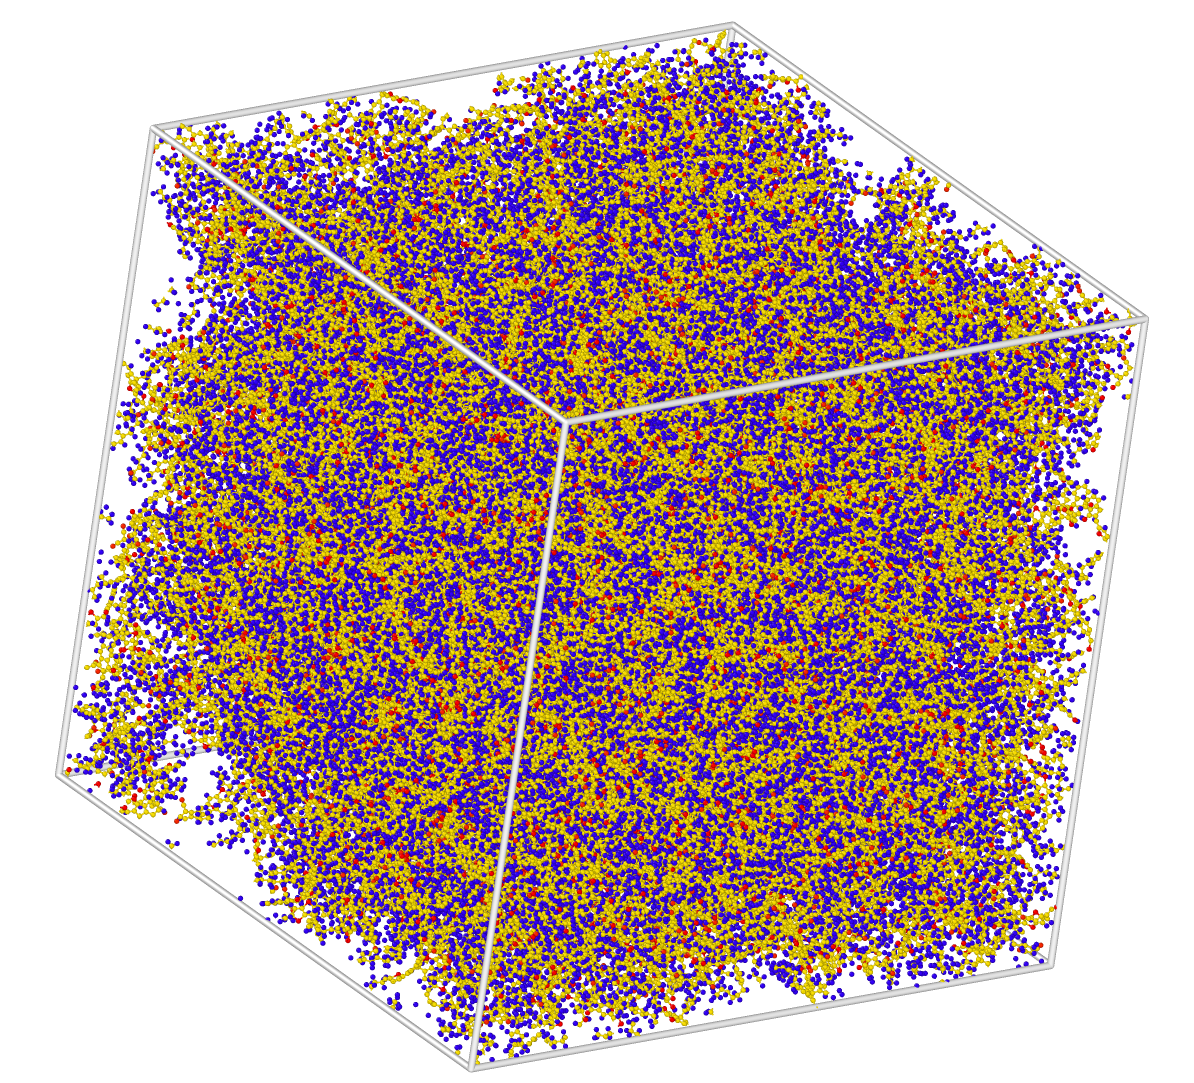
\includegraphics[width=\textwidth]{figures/ITIC.png}
\end{subfigure}%
\begin{subfigure}{.5\textwidth}
    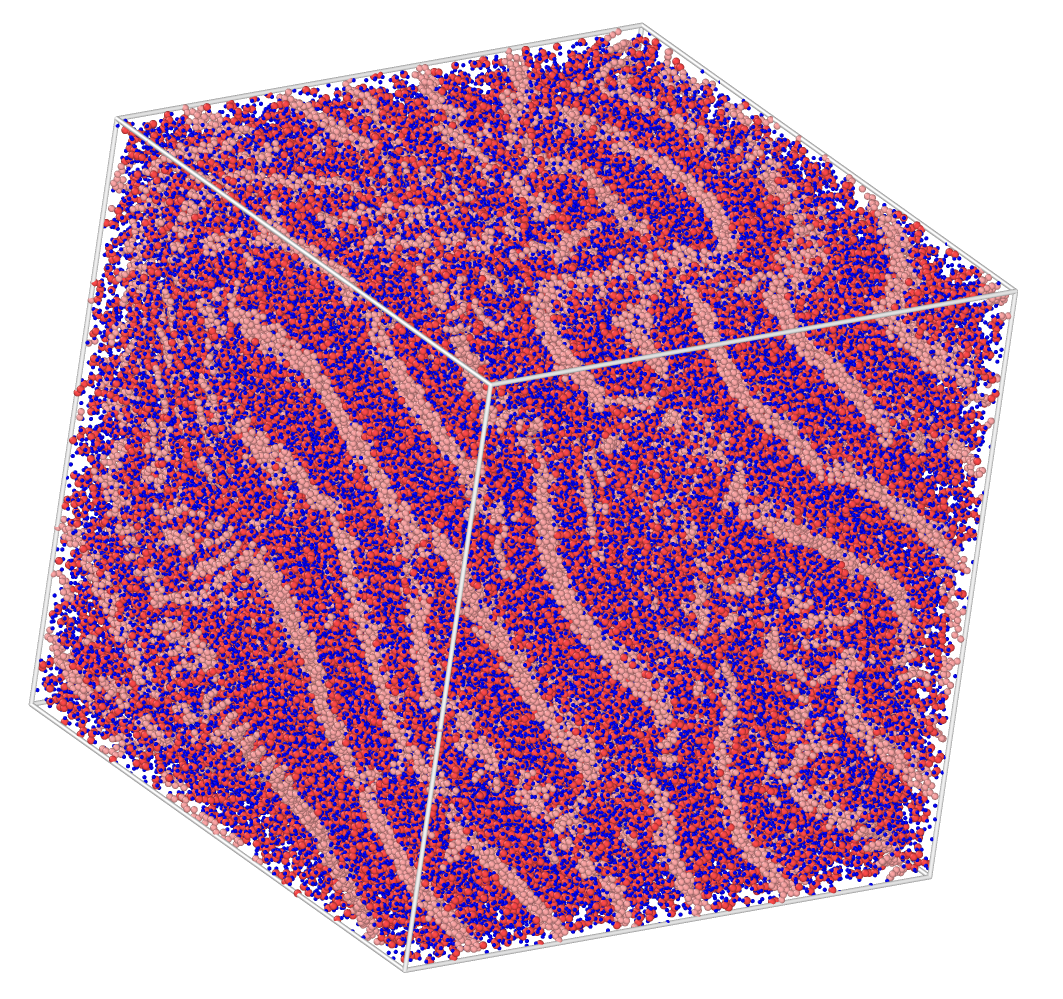
\includegraphics[width=\textwidth]{figures/P3HT.png}
\end{subfigure}
    \caption[short]{Left: 1000 molecule atomistic morhology of ITIC. Right: 1000 molecule atomistic simulation
    of P3HT}
\label{ITIC/P3HT}
\end{figure}


Two major breakthroughs have ushered us into the modern era of OSCs,
wherein effeciencies are approaching 20\% \cite{Liu2020b},
a value considered to be a critical mass beyond which the technology will be considered commercially viable.\ej{Cite needed}
These are the design of bulk heterojunction active layers and non-fullerene acceptor molecules. \ej{expecting examples of how BHJ's were one breakthrough and how NFAs were another}

In organic materials, the coloumbic attraction, $V$,  between the excited
electron and the hole it left behind in the its molecular orbital
is given by Coulombs law as follows:

\begin{align}
    V  =  k_{e} \cdot \frac{e^{2}}{\epsilon_{r}}
\end{align}

where $k_{e}$ is Coulomb's constant and $e$ is charge of an electron. The relative permitivitty,
$\epsilon_{r}$, of a material describes how readily a material
will polarize in response to an electric field, relative to readily free space will polarize. In OPVs a
relative permitivitty of $~3$ means that this material is 3 times more polarizable than free space, which
is not all that polariazable. And with that, the material occupying the space between electron and hole
is not readily oreinting itself in the direction of the electric field created between them, which would
oppose the Coulombic attraction. Silicon has a relative
permitivitty of ~12. This bound electron-hole quasiparticle is refered to herein as an exciton.

This introduces a unique design challenge.
To extract a charge from the device, the electron and hole
must be coerced apart. This coercion can take place at the interface between donor and acceptor molecules,
where the slight offset in energy levels creates a charge transfer state wherein it is more
energetically favorable for the donor to undergo electron transfer with an adjacent acceptor than
it is to radiatively decay to its ground state and photoemit.
However, after photoabsorbtion, the exciton must to diffuse to this interface for the charge to be
extracted. An exciton can diffuse roughly 10nm(Clarke) before relaxing \cite{Clarke2010} \ej{Citation needed. There's some evidence from Bernie Yurke and others that excitons can travel further than 10nm in ordered morphologies, and so this 10nm number is an informed guess based on only opv materials (Maybe some articles by Darling or McGehee can unpack this?), and that perhaps our simulations can help us dispel if untrue.}
Producing a layer this small is untenable and further a thicker layer
is diserable to interact with as much of the ambeint radiation as possible so as to ``catch'' as many photons
as possbible. 

In 1986, Ching W. Tang
showed that, processed under the right conditions, a blend of donor and acceptor molecules can self-assemble
into what is termed Bulk Heterojunction (BHJ) microstructure \cite{Tang1986c}. 
The interlocking phases of donor accepter molecules, ensure
that an exciton will intersect with the boundary between accepter and donor domains, while also ensuring that
there
is a continuous escape route, albeit labyrinthine, for the charges to travel on their way to their respective
electrodes. \ej{picture?} \ej{I didnt know if this meant real picture of bhj schematic but i made the latter
to refer to here as well as when i discuss the four stages of bhj}

\begin{figure}
    \center
    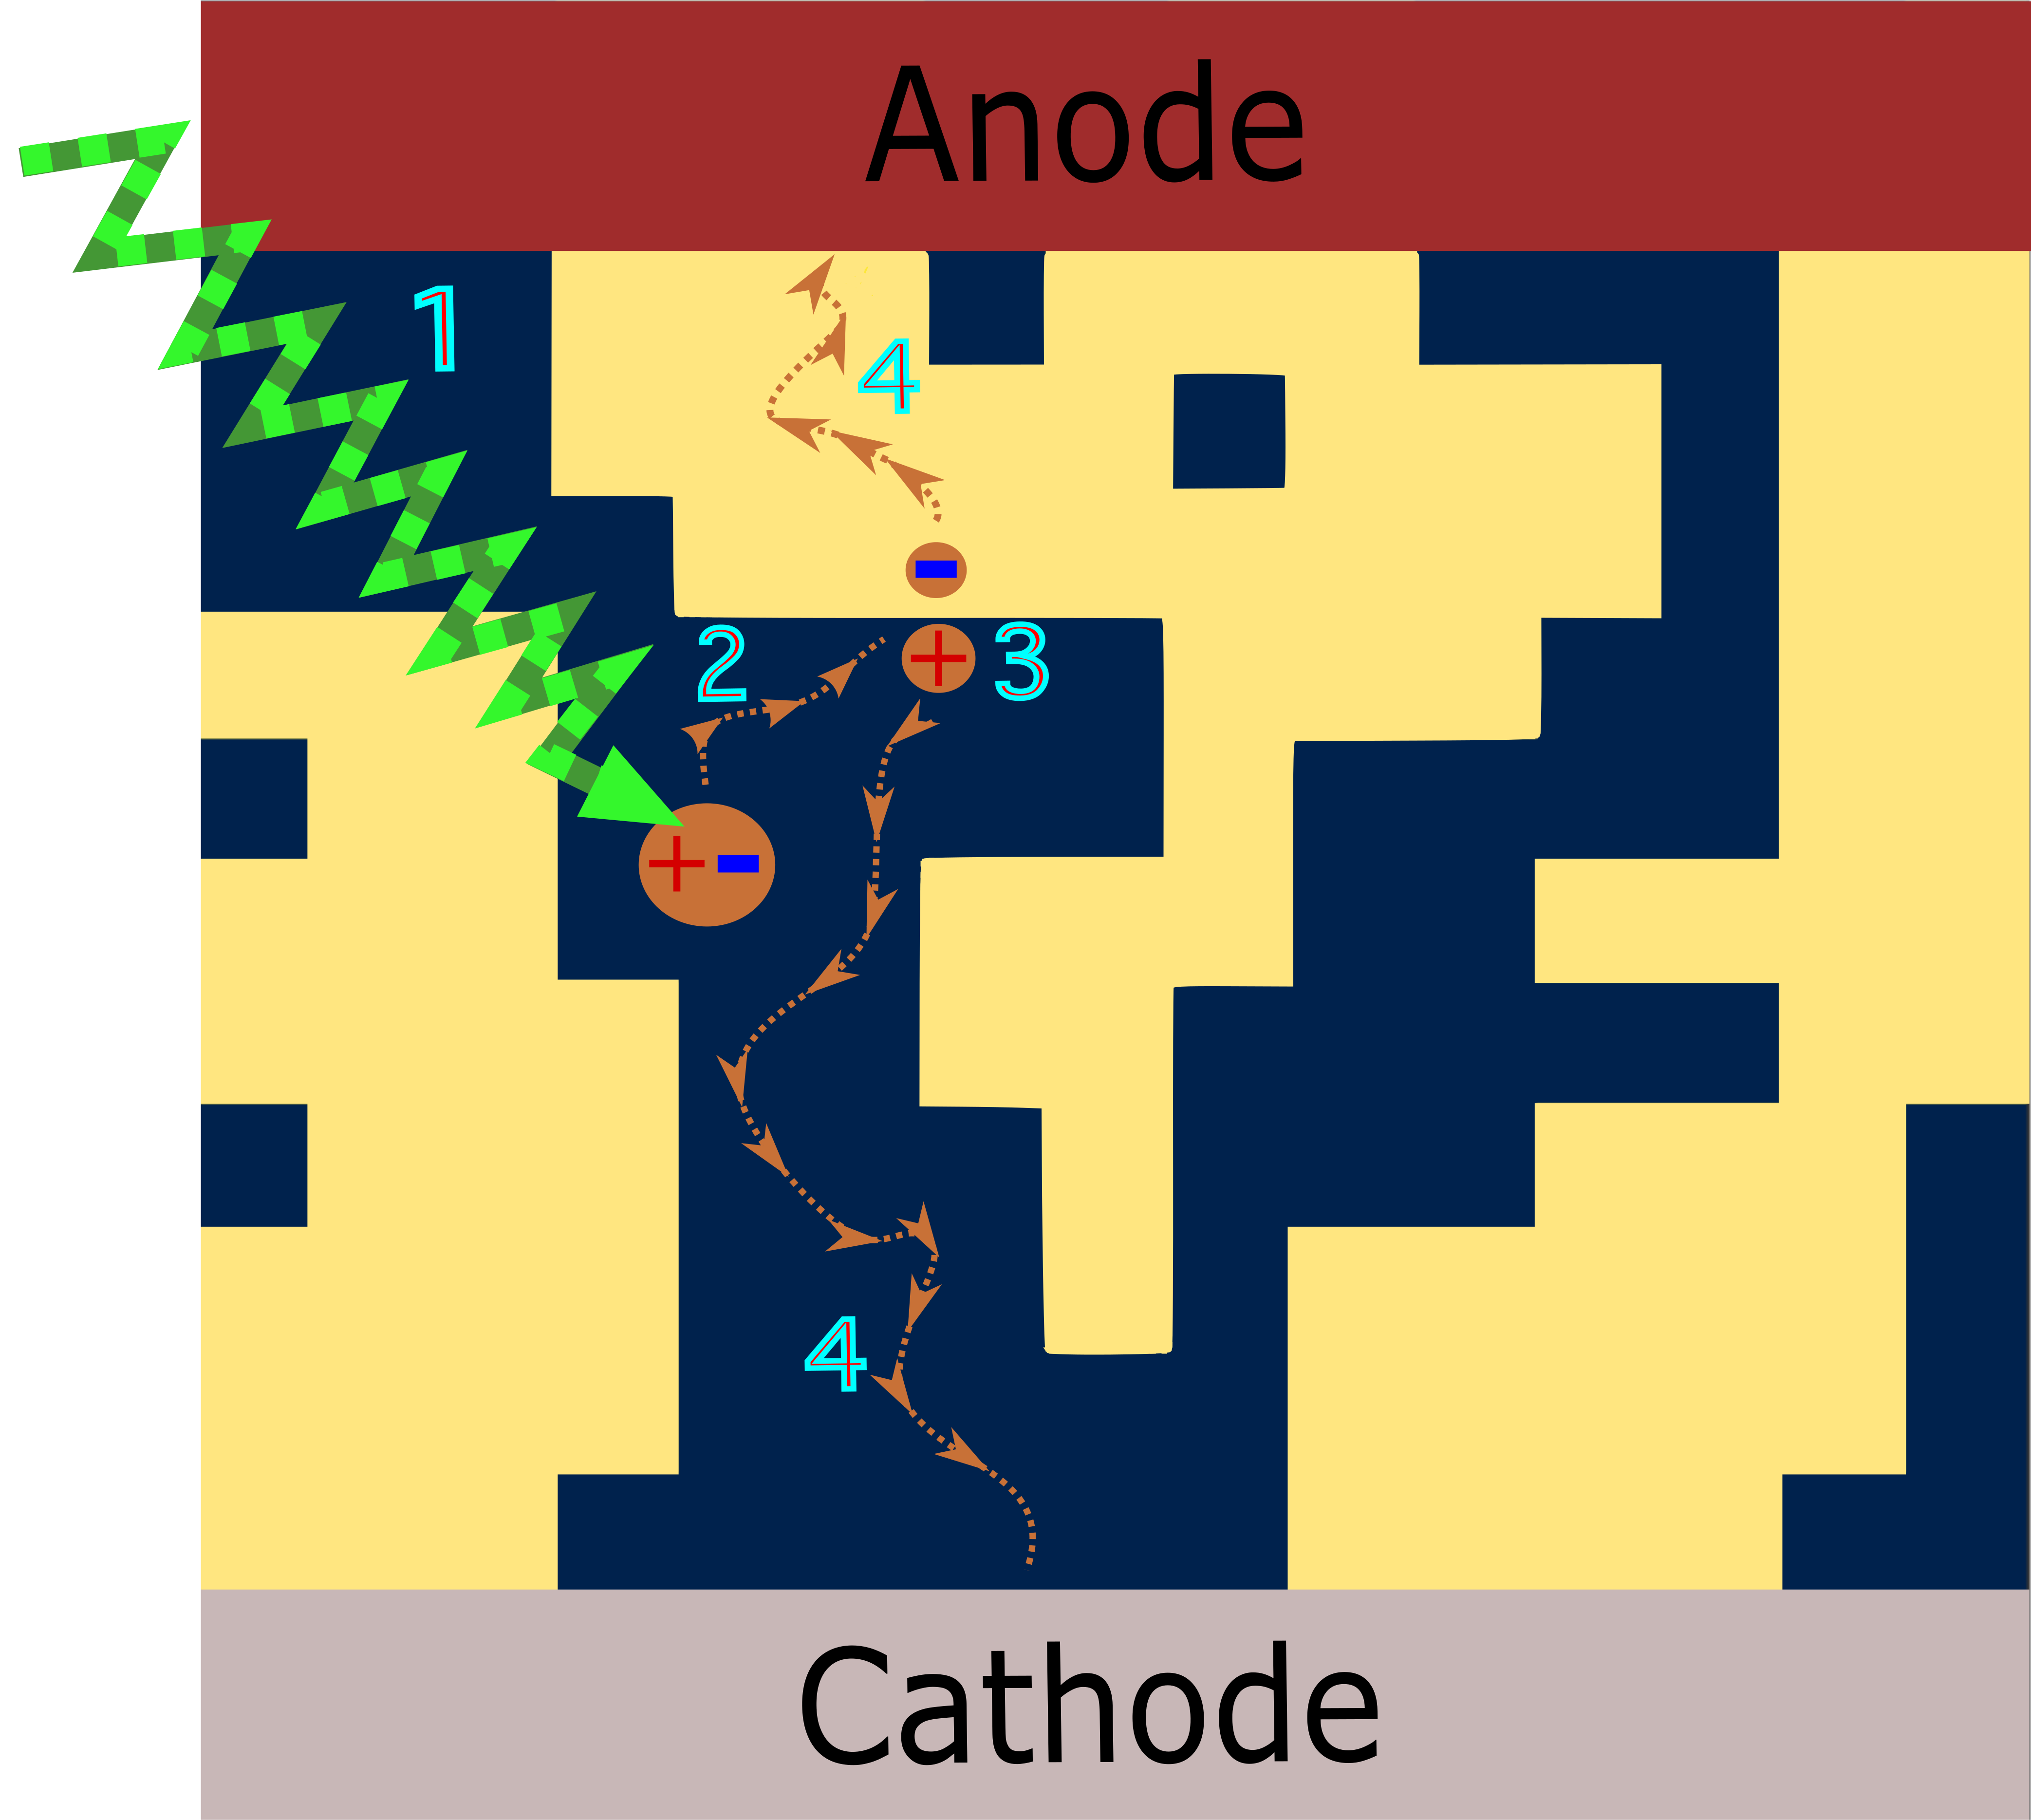
\includegraphics[width = .9\textwidth]{figures/BHJ-figure.png}
    \caption{A cartoon representation of a bulk heterojunction device. All four stages involved in harvesting
    photonic energy in a BHJ device are represtented. (1) The photon (green arrow) interacts with the material,
    exciting an electron and creating an quasiparticle referred to as an exciton. (2) The exciton diffuses
    about until it intersectects the interface between donor and acceptor material domains. (3) The exciton is
    coerced apart by the energy offset between donor and acceptor molecules. 
    (4) The, now unbound,  hole and the electron are free to diffuse about until ther reach their respective
    electrodes where they can be extracted}
    \label{bhj}
\end{figure}


Reaching 17 \% effeciency in these devices required rigorous theory and time consuming chemical synthesis
that unfolded over the course of three decades. \ej{How'd theory play a role?} 
With the immensity of parameter space involved in the design of BHJ material, it is desirable that a modular
open-source pipeline exhist for simulating the morphology of candidate molecules as well as simulating the 
associated charge charecteristics.\ej{Love it, but this is whiplash from the previous sentence. If we're pivoting to pipelines and screening now, then BHJ and NFA discussion is missing. I think maybe this sentence belongs elsewhere.} 
We note that will motivate zero-field mobility as a relvant quantity in BHJ
design, it could likely be informative accross all of the aforementioned applications. 


BHJ OSC work in 4 steps . photoabsorbtions, exciton diffusion, CT , Charge diffusion. \citet{Fusella2019}. \ej{Nice- still on BHJ and explaining physics is good.}
Engineering the active layer of an OSC from organic materials presents distinct challenges and advantages at
all four stages. 
Our work is expressely related to stage four. That is, after the photon has been absorbed, creating and
exciton that has diffused to the interface between donor and acceptor molecule, and the exciton has decoupled
coulumbically.\ej{Like above, a bit of whiplash. Maybe get through all this intro first, and THEN explain where our work fits in.} Now, with the free electron bouncing around in the acceptor domain (the hole in the donor) how
quickly will it diffuse in that environement? This diffusivity, charge mobility, is what can be characterized in experiments and simulations and is one key metric for overall device efficiency.
%using MorphCT.

It has been show that the hole/electron mobility of both donor and acceptor material are
relavant to overall device performance. \cite{Wang2019e}. If electron mobililty is too high
in acceptor \ej{confusing} in comparison to the hole mobility in the donor, it gets clogged up and you get 
nongeminate recombination loss\ej{define?}.
Also, imbalanced charge-carrier mobility can lead to space-charge build up in the low mobilty material that
can screen the built in field.  \cite{Bartelt2015}. \ej{picture?}

This phenomena has been shown by space charge limited current eperiments \cite{Small2013}.
Taking for granted that electronic devices utilizing organic materials are an exciting
space, \ej{Maybe this is the right place to pivot to motivation for the current work. If so, great!} we find it highly desirable to have a pipeline through which we can simulate the equilibrium
chemistries of these materials and characterize their emergent material properties. Jones2017 has laid out this
pipeline in detail from the use of molecular dynamics simulations to predict the chemical structure to the use
if Kinetic Monte Carlo simulations to characterize charge mobility (conductivity) in these chemistries.
\ej{Perhaps this is the place for a picture of the pipeline in terms of techniques/theory used, and we can get into our specifics later?}

\ej{This paragraph maybe belongs after the generic workflow description?}
Two open source python packages, Planckton and MorphCT, are maintained at https://github.com/cmelab for
facilitating these two legs of the pipeline. The use of Planckton in the methods and results sections below
constitute the experience of an end user as I had not personally developed this package before conscripting it
to do my MD simulating. Using Planckton-flow (also maintained on github), a sister package
of Planckton we took a container of planckton off the shelf and ran MD simulations of benchmark OPV
molecules on a high performance computing cluster without having to build the software stack or write the
simulation scripts from scratch. 

\ej{Need explanation of TRUE}
My experience evinces what TRUE simulation engines can achieve and
informs the direction with which we seek to take MorphCT. We hope that the combination of these two packages
can make in silico experimentation with these materials realistically attainable by any aspiring researcher.
Having had no prior experience with these materials and/or materials simulation prior to joining the CMElab,
I was able to take an investigation of ITIC from molecular
structure to a charge mobility; a macroscopic property. 

Version one of MorphCT was capable of
connecting qualitativley the morphological features produced by MD simulations. However, it was determined
that in the interest of reprducabitilty, it was critical to ``containerize'' this pipeline. Until as recently as
the past few years it was common place to not publish code with the results of computational works. Containers
are virtual machines that contain all the dependencies, configurations, code and data necessary to reproduce
results. \cite{Cito2016a}

THIS SENTECE HAS NO HOME Researchers have to
balance the optimiztion of electron structures of candidate donor/acceptor materials against the miscibility
of two candidate molecules as well as the resultant morphology across the thermodynamic landscape of
variuos solution processes which ultimately govern the Jsc and FF of at the device level \cite{Zhu2020a}. 
\ej{After we show the generic pipeline of calculations that are needed, I think this is where we explain what specifically we do here: ``In this work we develop X for Y. In Section 2 we describe the theory and specific implementations of the methods used throughout the pipeline. In section 3 we report on experiments for validating and verifying our methods. In Section 4 we discuss the ramifications of this work and detail areas of future work.''}
%%% Local Variables: 
%%% mode: latex
%%% TeX-master: "BSUmain"
%%:set textwidth=80
% End: 
